
\begin{enumerate}
\item Tracer la courbe de la fonction Inverse en affichant un pas convenable en ordonnée.




\item  Dresser le tableau de variation de la fonction Inverse.

\begin{tikzpicture}
\tkzTabInit[lgt=1,espcl=2]{ $x$ / 1,$f $ / 2}
{ $-\infty$ , $0$ ,$+\infty$}
\tkzTabVar{+/$0$ , -D+ /$ $/$ $ , -/$0$}
\end{tikzpicture}

\item  Tracer les droites d'équation $y=\frac{1}{2}$ et $y=-3$.

\definecolor{ffqqqq}{rgb}{1.,0.,0.}
\definecolor{qqqqff}{rgb}{0.,0.,1.}
\definecolor{qqwuqq}{rgb}{0.,0.39215686274509803,0.}
\begin{tikzpicture}[line cap=round,line join=round,>=triangle 45,x=0.8393694192461024cm,y=1.463130573525573cm]
\begin{axis}[
x=0.8393694192461024cm,y=1.463130573525573cm,
axis lines=middle,
ymajorgrids=true,
xmajorgrids=true,
xmin=-8.226309222060465,
xmax=10.450084686994161,
ymin=-3.2121167225373934,
ymax=1.1063198358073438,
xtick={-8.0,-7.0,...,10.0},
ytick={-3.0,-2.0,...,1.0},]
\clip(-8.226309222060465,-3.2121167225373934) rectangle (10.450084686994161,1.1063198358073438);
\draw[line width=2.pt,color=qqwuqq,smooth,samples=100,domain=-8.226309222060465:10.450084686994161] plot(\x,{1.0/(\x)});
\draw [line width=2.pt,color=qqqqff,domain=-8.226309222060465:10.450084686994161] plot(\x,{(--0.5-0.*\x)/1.});
\draw [line width=2.pt,color=ffqqqq,domain=-8.226309222060465:10.450084686994161] plot(\x,{(-3.-0.*\x)/1.});
\draw (-5.458031546200592,1.0582303418391397) node[anchor=north west] {$ \textcolor{blue} {y=\frac1 2}$};
\draw (-5.420109934202512,-2.625424896125302) node[anchor=north west] {$\textcolor{red}{y=-3}$};
\begin{scriptsize}
\draw[color=qqwuqq] (-9.269153552007678,-0.16805175435006758) node {$f$};
\draw[color=qqqqff] (-9.269153552007678,0.4282579708556645) node {$g$};
\draw[color=ffqqqq] (-9.269153552007678,-2.8322097201885805) node {$h$};
\end{scriptsize}
\end{axis}
\end{tikzpicture}


\item  Déterminer graphiquement le(s) antécédent(s) de  $\frac{1}{2}$ par la fonction Inverse.

Le(s) antécédent(s) de  $\frac{1}{2}$ par la fonction Inverse sont les abscisses des points d'intersection de la courbe avec la droite d'équation $y=\frac{1}{2}$. Donc il y a un seul antécédent à $\frac{1}{2}$ par la fonction Inverse, c'est \fbox{$x=2$}.

\item  On appelle $g$ la fonction Inverse. Résoudre graphiquement $g(x)=-3$.

Résoudre graphiquement $g(x)=-3$ revient à déterminer les abscisses des points d'intersection de la courbe avec la droite d'équation $y=-3$. Donc il y a un seul antécédent à $-3$ par la fonction Inverse $g$, c'est $x=-\frac{1}{3}$. \fbox{$S = \lbrace -\frac{1}{3}\rbrace$}.

\item  Résoudre par le calcul $g(x)=-3$. Valider le résultat avec la courbe .

$g(x)=-3 \Longleftrightarrow \frac{1}{x} = -3 \Longleftrightarrow x=-\frac{1}{3}$. \fbox{$S = \lbrace -\frac{1}{3}\rbrace$}.


\item  Déterminer graphiquement $g(x)\leq \frac{1}{2}$.

Résoudre graphiquement $g(x)\leq \frac{1}{2}$ revient à déterminer les abscisses des points de la courbe en dessous de la droite d'équation $y=\frac{1}{2}$. \fbox{$S=\left]-\infty;0 \right[ \cup \left[2;+\infty \right[ $}.

 
\item  Déterminer graphiquement $-3 \leq \frac{1}{x} \leq \frac{1}{2}$. 

Résoudre graphiquement $-3 \leq \frac{1}{x} \leq \frac{1}{2}$ revient à déterminer les abscisses des points de la courbe en-dessous de la droite d'équation $y=\frac{1}{2}$ \textbf{et} au-dessus de la droite d'équation $y=-3$. 

\fbox{$S=\left]-\infty;-\frac{1}{3}  \right[ \cup \left[2;+\infty \right[ $}.



\item  Résoudre par le calcul $-3 \leq \frac{1}{x} \leq \frac{1}{2}$. On procédera par disjonction de cas.




\begin{enumerate}

\item  Résoudre par le calcul $-3 \leq \frac{1}{x} $.

$-3 \leq \frac{1}{x} \Longleftrightarrow  0 \leq \frac{1}{x}+3  \Longleftrightarrow  0 \leq \frac{1+3x}{x} $

\begin{tabular}{|c|ccccccc|}
\hline 
$x$ & $-\infty$ &   & $-\frac{1}{3}$ &  & 0 & & $+\infty$ \\ 
\hline 
$x$ &  & $-$ &  & $-$   & 0 & $+$ &  \\ 
\hline 
$1+3x$ &  & $-$ & 0 & 0 & $+$ & $+$ & \\ 
\hline 
$\frac{1+3x}{x}$ &  & $+$ & 0 &$-$ & $\Vert$ & $+$ &  \\ 
\hline 
\end{tabular} 

$S_1=\left]-\infty;-\frac{1}{3}  \right] \cup \left]0;+\infty \right[ $


\definecolor{ffqqqq}{rgb}{1.,0.,0.}
\definecolor{xdxdff}{rgb}{0.49019607843137253,0.49019607843137253,1.}
\begin{tikzpicture}[line cap=round,line join=round,>=triangle 45,x=1.8645607217854918cm,y=1.0cm]
\begin{axis}[
x=1.8645607217854918cm,y=1.0cm,
axis lines=middle,
xmin=-2.615780920496802,
xmax=3.167502860512811,
ymin=-0.3669181545954532,
ymax=0.2686769681740082,
xtick={-2.0,-1.0,...,3.0},
ytick={-0.0,1.0,...,0.0},]
\clip(-2.615780920496802,-0.3669181545954532) rectangle (3.167502860512811,0.2686769681740082);
\draw [line width=2.pt,color=ffqqqq,domain=0.0:3.167502860512811] plot(\x,{(-0.-0.*\x)/8.59844023594419});
\draw [line width=2.pt,color=ffqqqq,domain=-2.615780920496802:-0.3251222738292293] plot(\x,{(-0.-0.*\x)/-4.674877726170771});
\begin{scriptsize}
\draw [fill=xdxdff] (8.59844023594419,0.) circle (2.5pt);
\draw [fill=ffqqqq] (-0.3251222738292293,0.) circle (2.5pt);
\draw [fill=xdxdff] (-5.,0.) circle (2.5pt);
\end{scriptsize}
\end{axis}
\end{tikzpicture}




\item  Résoudre par le calcul $\frac{1}{x} \leq \frac{1}{2}$

$\frac{1}{x} \leq \frac{1}{2} \Longleftrightarrow  \frac{1}{x} - \frac{1}{2} \leq 0  \Longleftrightarrow    \frac{2-x}{2x} \leq 0$

\begin{tabular}{|c|ccccccc|}
\hline 
$x$ & $-\infty$ &   & $0$ &  & 2 & & $+\infty$ \\ 
\hline 
$2x$ &  & $-$ & 0 &  $+$  &  & $+$ &  \\ 
\hline 
$2-x$ &  & $+$ &   & $+$ & 0 & $-$ & \\ 
\hline 
$\frac{1+3x}{x}$ &  & $-$ & $\Vert$ & $+$ & 0 & $-$ &  \\ 
\hline 
\end{tabular} 

$S_2=\left]-\infty;0  \right[ \cup \left[2;+\infty \right[ $


\definecolor{qqqqff}{rgb}{0.,0.,1.}
\definecolor{xdxdff}{rgb}{0.49019607843137253,0.49019607843137253,1.}
\begin{tikzpicture}[line cap=round,line join=round,>=triangle 45,x=1.0cm,y=1.0cm]
\begin{axis}[
x=1.0cm,y=1.0cm,
axis lines=middle,
xmin=-2.628366957016953,
xmax=3.394051517875538,
ymin=-0.2662298183151425,
ymax=0.20574675799881403,
xtick={-2.0,-1.0,...,3.0},
ytick={-0.0,1.0,...,0.0},]
\clip(-2.628366957016953,-0.2662298183151425) rectangle (3.394051517875538,0.20574675799881403);
\draw [line width=2.pt,color=qqqqff,domain=2.0:3.394051517875538] plot(\x,{(-0.-0.*\x)/1.});
\draw [line width=2.pt,color=qqqqff,domain=-2.628366957016953:0.0] plot(\x,{(-0.-0.*\x)/-3.});
\begin{scriptsize}
\draw [fill=xdxdff] (8.59844023594419,0.) circle (2.5pt);
\draw [fill=xdxdff] (-5.,0.) circle (2.5pt);
\draw [fill=xdxdff] (2.,0.) circle (2.5pt);
\draw [fill=xdxdff] (-3.,0.) circle (2.5pt);
 
\end{scriptsize}
\end{axis}
\end{tikzpicture}



On veut alors à la fois les deux solutions. C'est à dire la partie à la fois bleue et rouge.
 

\definecolor{ududff}{rgb}{0.30196078431372547,0.30196078431372547,1.}
\definecolor{qqqqff}{rgb}{0.,0.,1.}
\definecolor{ffqqqq}{rgb}{1.,0.,0.}
\definecolor{xdxdff}{rgb}{0.49019607843137253,0.49019607843137253,1.}
\begin{tikzpicture}[line cap=round,line join=round,>=triangle 45,x=1.0cm,y=1.0cm]
\begin{axis}[
x=1.0cm,y=1.0cm,
axis lines=middle,
xmin=-2.3451811353135446,
xmax=3.2052609700732657,
ymin=-0.21588565017498712,
ymax=0.23721186308641112,
xtick={-2.0,-1.0,...,3.0},
ytick={-0.0,1.0,...,0.0},]
\clip(-2.3451811353135446,-0.21588565017498712) rectangle (3.2052609700732657,0.23721186308641112);
\draw [line width=2.pt,color=ffqqqq,domain=0.0:3.2052609700732657] plot(\x,{(-0.-0.*\x)/8.59844023594419});
\draw [line width=2.pt,color=ffqqqq,domain=-2.3451811353135446:-0.3251222738292293] plot(\x,{(-0.-0.*\x)/-4.674877726170771});
\draw [line width=2.pt,color=qqqqff,domain=2.0:3.2052609700732657] plot(\x,{(--0.4-0.*\x)/4.});
\draw [line width=2.pt,color=qqqqff,domain=-2.3451811353135446:0.0] plot(\x,{(-0.3-0.*\x)/-3.});
\begin{scriptsize}
\draw [fill=xdxdff] (8.59844023594419,0.) circle (2.5pt);
\draw [fill=ffqqqq] (-0.3251222738292293,0.) circle (2.5pt);
\draw [fill=xdxdff] (-5.,0.) circle (2.5pt);
\draw [fill=xdxdff] (2.,0.1) circle (2.5pt);
\draw [fill=xdxdff] (-3.,0.1) circle (2.5pt);
\end{scriptsize}
\end{axis}
\end{tikzpicture}

donc $S=S_1 \cap S_2 = \left]-\infty;-\frac{1}{3}  \right] \cup \left[2;+\infty \right[ $

\textbf{Attention aux crochets !}
\end{enumerate}

\end{enumerate}
